% --------------------------------------------------------------
% Abhi's Standard Preamble.
% --------------------------------------------------------------
 
\documentclass[12pt]{article}
 
%Packages
\usepackage[margin=1in]{geometry} 
\usepackage{graphicx}
\usepackage{url}
\usepackage{hyperref}
\usepackage{float}
\usepackage{quoting}

\usepackage{aurical}
 
\begin{document}
 
\title{ACC-72}
\date{}

\maketitle

\begin{figure}[!htb]
  \centering
  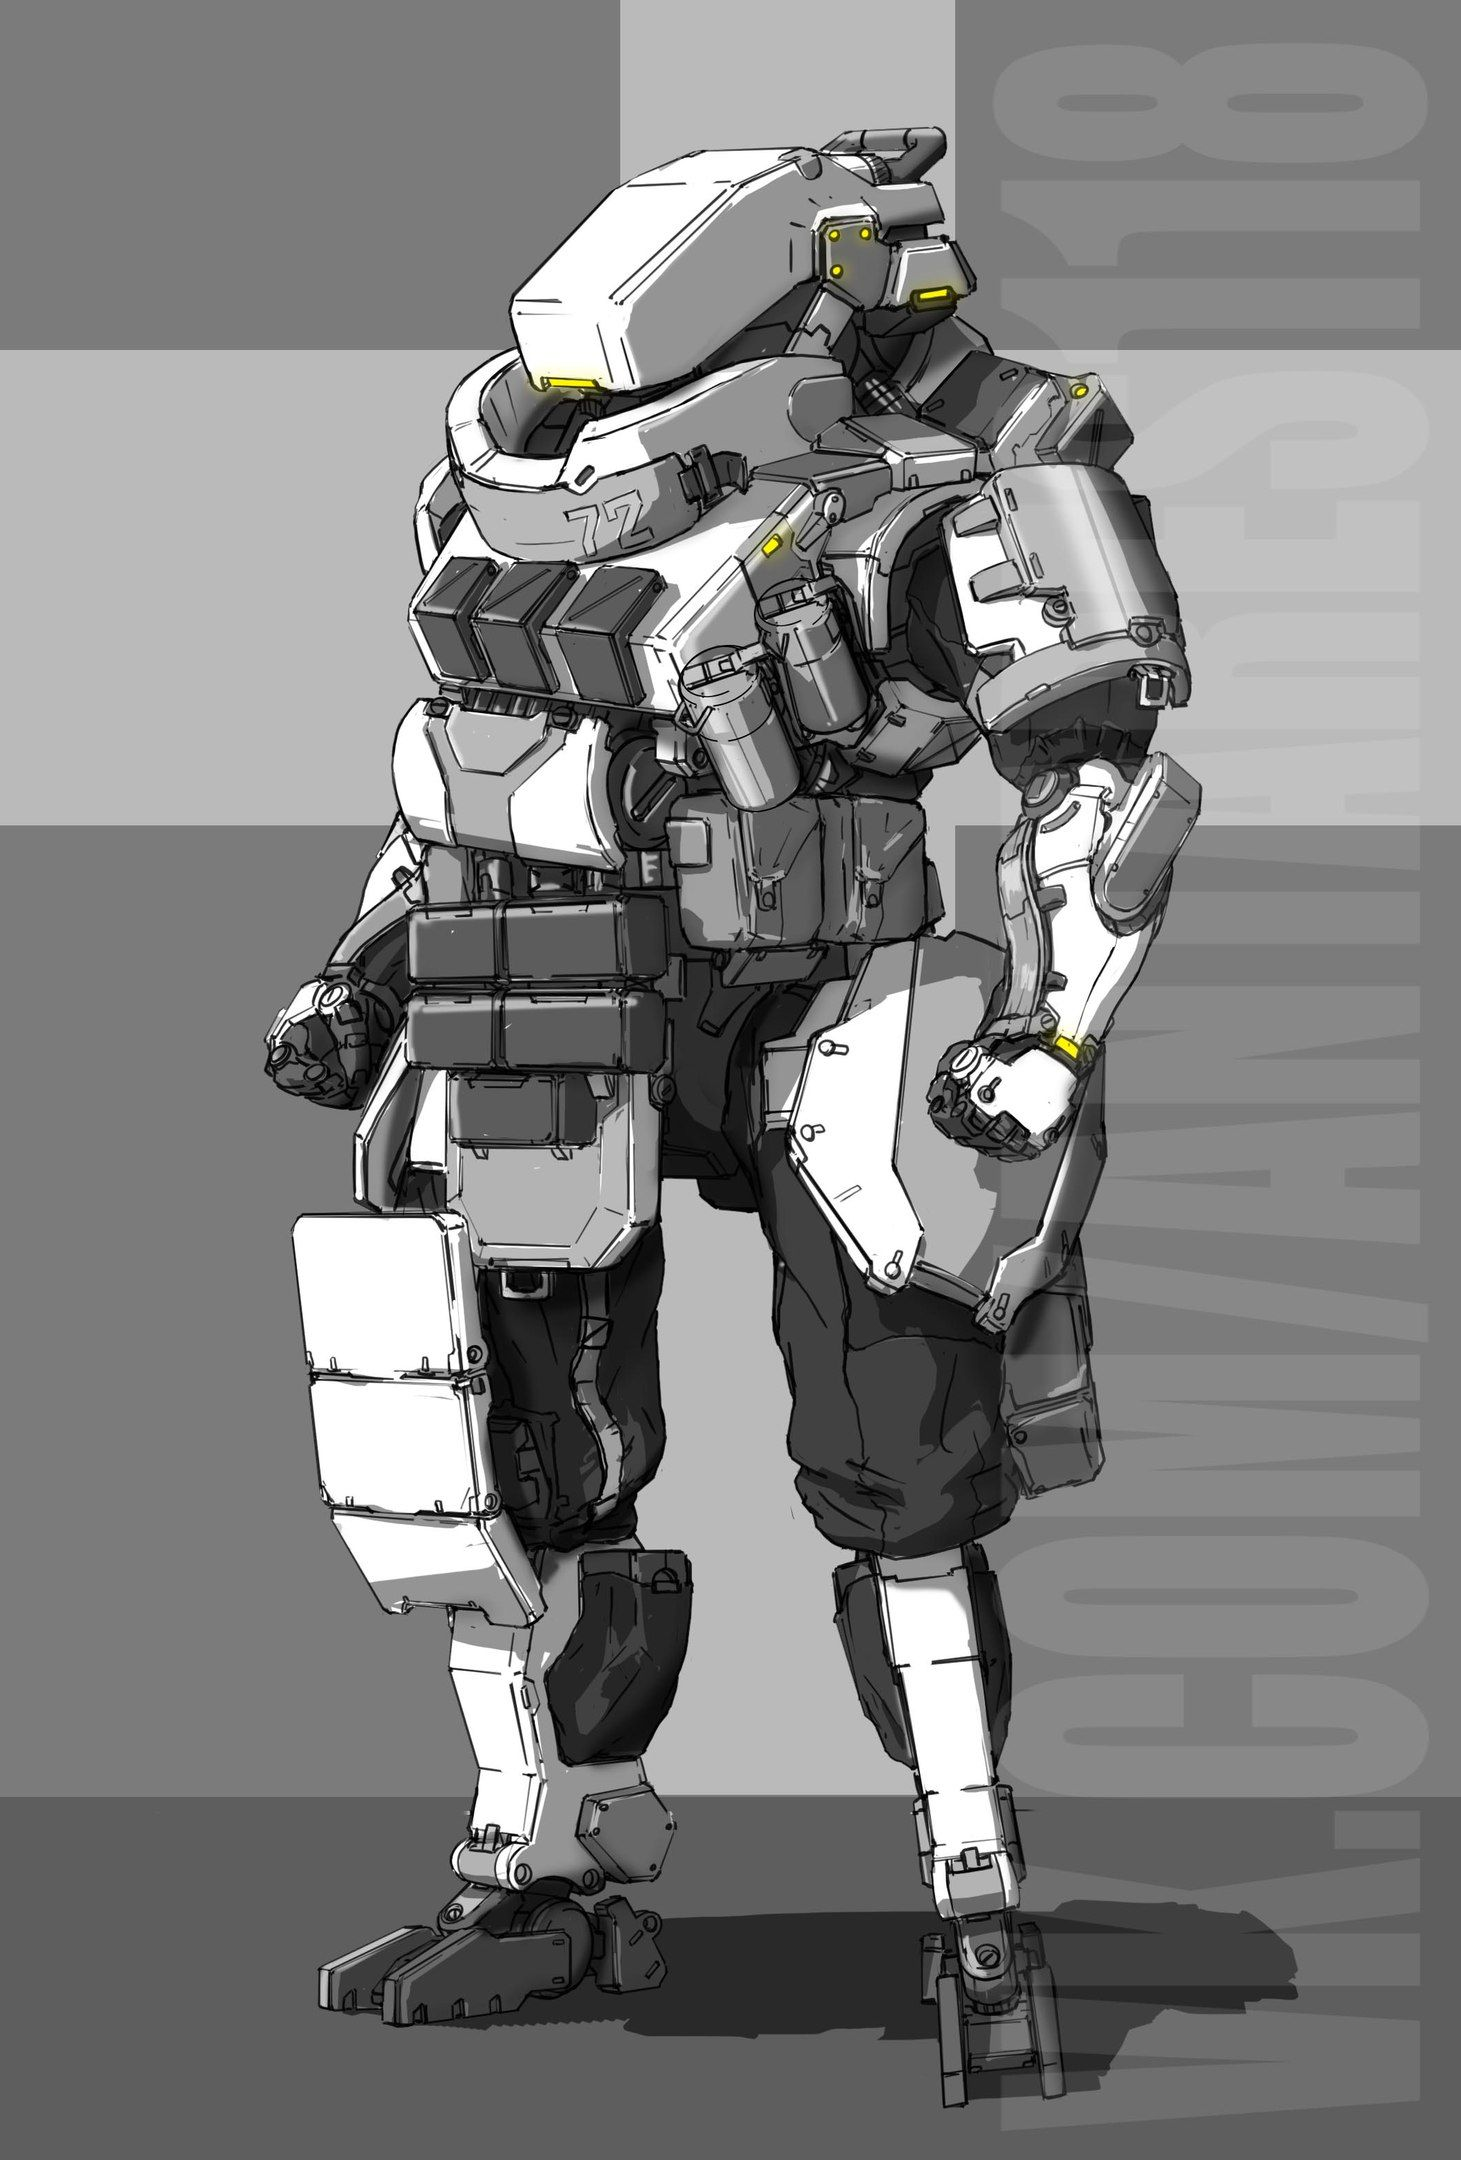
\includegraphics[width=.68\textwidth]{./resources/acc72}
  \caption{ACC-72 in his battle armor.}
\end{figure}

\section{Character Description}

A droid seemingly of the class four variety, ACC-72 is built for war. 
Covered in thick durasteel armor, the droid's figure is hulking and
intimidating, standing 8 feet tall and weighing a massive 720 pounds. 
On his back he carries two large weapons. 
The first is a massive assault cannon, not unlike the weapons used by the heavy
soliders of both the Imperial and Galactic armies, and the second is an
comparatively smaller ion rifle. 
Both have a scratched out insignia and an innumerable amount of notches scraped
into it, and you would have seen ACC-72 notch another for each kill. 
His armor contains slots for additional equipment to be carried, such as
grenades and other armaments, but they are currently empty. 
ACC-72 typically dons a cloth-spun cloak, which he refuses to part with no
matter how dirty and damaged it gets. 
He personally takes up the maintainance of it, even going to lengths to find
and obtain large quantities of the original material so he could repair it.
He keeps the hood up, although it does little to conceal his non-humanoid head
and the green LEDs underneath. 
Owing to his large size, his gait appears to be slow, heavy, and methodical. 

\begin{figure}[!htb]
  \centering
  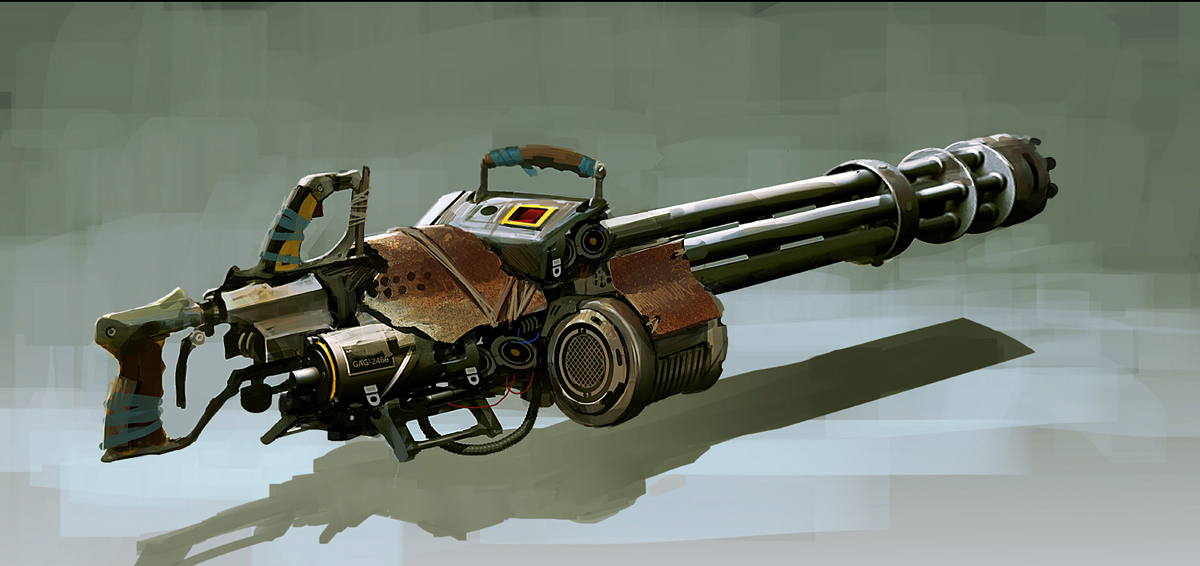
\includegraphics[width=.7\textwidth]{./resources/assaultcannon}
  \caption{The assault cannon that ACC-72 wields}
\end{figure}

ACC-72 is usually quiet and polite to those who would interact with him.
Prefering to answer in cryptic and short sentences, words are a commodity when
conversing with him, although he doesn't mean to deliberately confuse. 
This standoffish behavior, however, is dropped when he finds something
interesting, instead ceaselessly questioning and pondering on the subject, often
to the annoyance of the subject in question. 
This behavior, unnatural given his size and normal demeanor, is likely a glitch
or personality trait developed after going an unknown amount of time without
a memory wipe. 
With regards to things that interest him, ACC-72 is intensely curious about the
weapons of the galaxy, wishing to hoard and collect them, in addition to
upgrading his own.

Likely originally built as a defensive droid, his armor incorporates a personal
barrier and he is equipped with many protective battle routines. 
His reward receptors are triggered when he protects someone from danger, and he
has turned that desire into his role among his party, as the steadfast bulwark
protecting them from danger. With this in mind, ACC-72 feels very anxious
without atleast one of his party members nearby. 
It's unknown exactly how this role as a protector fits in with his obsession
with arms.

\section{Backstory}

\section{Relations}

\subsection{Ellara Veil}

\subsection{Aranar Ordo}

\subsection{Padawan Kusk}

\subsection{Una'More}

\end{document}
